%
% schnittkurven.tex
%
% (c) 2025 Prof Dr Andreas Müller, OST Ostschweizer Fachhochschule
%
\documentclass[tikz]{standalone}
\usepackage{times}
\usepackage{amsmath}
\usepackage{txfonts}
\usepackage[utf8]{inputenc}
\usepackage{graphics}
\definecolor{darkgreen}{rgb}{0,0.6,0}
\definecolor{darkred}{rgb}{0.8,0,0}
\definecolor{basisblau}{rgb}{0.0,0.2,1.0}
\usetikzlibrary{arrows,intersections,math}
\usepackage{ifthen}
\begin{document}

\newboolean{showgrid}
\setboolean{showgrid}{false}
\def\breite{7}
\def\hoehe{4}

\begin{tikzpicture}[>=latex,thick]

\clip (-6.3,-3.55) rectangle (6.3,3.55);

% Povray Bild
\node at (0,0) {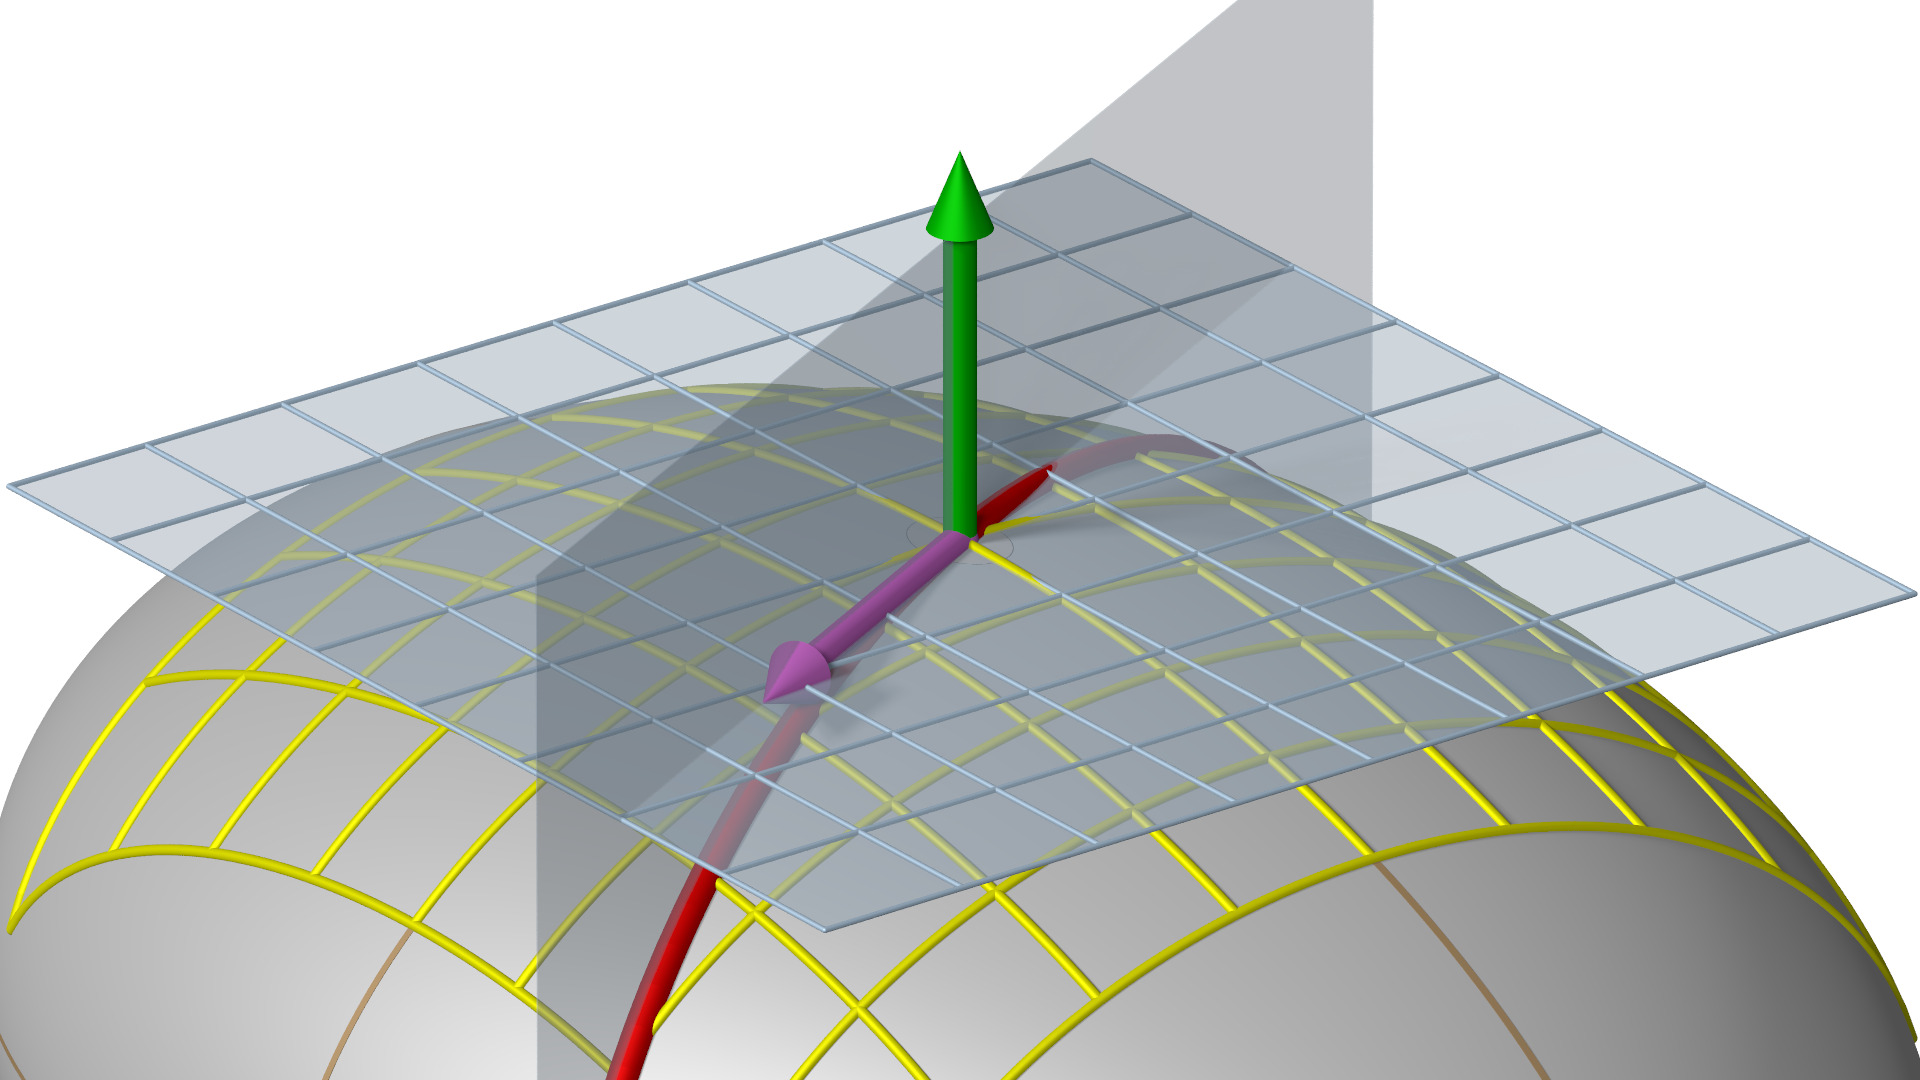
\includegraphics[width=12.6cm]{schnittkurven.jpg}};

% Gitter
\ifthenelse{\boolean{showgrid}}{
\draw[step=0.1,line width=0.1pt] (-\breite,-\hoehe) grid (\breite, \hoehe);
\draw[step=0.5,line width=0.4pt] (-\breite,-\hoehe) grid (\breite, \hoehe);
\draw                            (-\breite,-\hoehe) grid (\breite, \hoehe);
\fill (0,0) circle[radius=0.05];
}{}

\node[color=darkgreen] at (-0.3,2.6) {$\vec{m}$};
\node[color=violet] at (-1.45,-0.9) {$\vec{t}$};
\node[color=darkred] at (-1.6,-3.3) {$\gamma(t)$};
\node[color=basisblau] at (-2.3,-0.4) {$\vec{r}_u$};
\node[color=basisblau] at (1.9,-0.7) {$\vec{r}_v$};

\end{tikzpicture}

\end{document}

